This layer processes the data scanned from the presentation layer and stores the data in local variables, i.e. name 
of the beverage and expiry date. This data is added to the current user's beverage database and send the updated data
back to the presentation layer for further input.

\subsection{API Subsystem}
The API subsystem passes the barcode to the Data Access Layer and retrieves the information of the beverage being 
scanned. The data retrieved is added to the current dataset of beverages which the user owns. 

\begin{figure}[h!]
	\centering
 	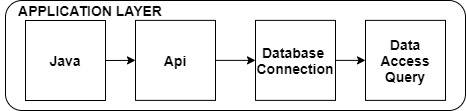
\includegraphics[width=0.60\textwidth]{images/App.jpg}
 \caption{Example subsystem description diagram}
\end{figure}

\subsubsection{Assumptions}
\begin{itemize}
    \item The drink is in the database of drinks.
    \item The data inputted is correctly scanned. 
\end{itemize}

\subsubsection{Responsibilities}
The data must be properly retrieved and stored to avoid glitches in teh application and ensure that the user 
is satisfied.

\subsubsection{Subsystem Interfaces}

\begin {table}[H]
\caption {Subsystem interfaces} 
\begin{center}
    \begin{tabular}{ | p{1cm} | p{6cm} | p{3cm} | p{3cm} |}
    \hline
    ID & Description & Inputs & Outputs \\ \hline
    \#1 & Appplication to Data Access & \pbox{Scanned Barcode ID} & \pbox{Product ID}  \\ \hline
    \#xx & Appplication to Presentation & \pbox{Data} & \pbox{Data in readable format}  \\ \hline
    \end{tabular}
\end{center}
\end{table}


